\documentclass[12pt,a4paper]{article}
\usepackage[utf8]{inputenc}
\usepackage{amsmath}
\usepackage{amsfonts}
\usepackage{enumitem}
\usepackage{amssymb}
\usepackage{graphicx}
\author{Anish Dalal}
\begin{document}
\begin{enumerate}
\item
\begin{enumerate}[label=(\alph*)]
\item Something interesting about the Berkeley Parser is how it judged the most probable parse of words based on contextual information. When we fed the parser sentences mixed with real words and gibberish words, the parser still assigned valid preterminals to the gibberish words based on the words surrounding it. For example, in the sentence ``My asdfjkasdjl went alksdf the store", the parser produced\\
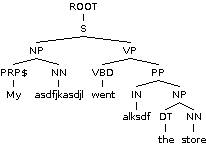
\includegraphics[scale=0.7]{gibparsetree}\\
where the gibberish words are assigned valid ``NN" preterminals. Another thing that was interesting was the parser was able to handle contractions i.e ``don't", ``can't".\\
\item Certain syntactic and lexically ambiguous statements caused the parser to produce an incorrect parse. The following lexically ambiguous sentence ``If police police police police, who police police police?" was parsed incorrectly by the Berkeley parser\\
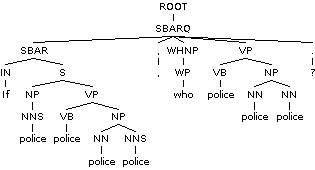
\includegraphics[scale=0.7]{policepoliceparsetree}\\
The way the sentence is structured, it is referring to a noun phrase ``police police" who are in charge of ``police". The sentence is saying ``If there are police officers who monitor other police officers who monitors those police officers?". The parser got the ``police police" noun phrase correct in the second half of the sentence but failed to recognize ``police police" as a noun phrase in the first half (it believes ``police" police ``police police", rather than ``police police" police ``police").  The parser does not handle garden path sentences very well either, however, it managed to produce the correct parse for ``The complex houses married and single soldiers and their families"\\
\includegraphics[scale=0.7]{soldiers}\\
where it correctly interpreted ``complex houses" not as a noun phrase but as a noun phrase followed by a verb phrase. \\
\item We created the grammatical sentence ``Buffalo run runs running runs". The sentence contains lexical ambiguity. It means ``Buffalo run while running". The phrase ``running runs" is a VP and an NP, so it should be created from the VP $\rightarrow$ VP NP rule. The parser incorrectly parses this\\
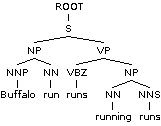
\includegraphics[scale=0.7]{buffalorun}\\
since it makes the phrase ``running runs" an NP.\\
We found the sentence ``The word of the Lord came to Zechariah, son of Berekiah, son of Iddo, the prophet". The ambiguity is that ``the prophet" can refer to either ``Iddo" or ``Zechariah" when in reality it refers to ``Zechariah" (this sentence is from the hebrew Bible). The parser believes the Iddo is the prophet rather than Zechariah\\
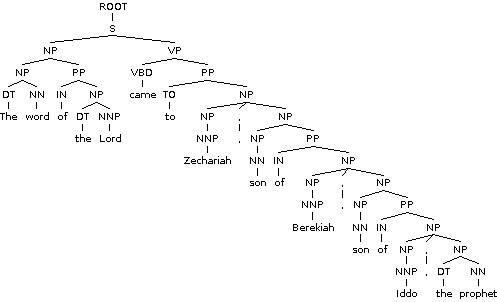
\includegraphics[scale=0.7]{zechariah}\\
where it creates a noun phrase for ``Iddo the prophet". \\
\end{enumerate}
\item
\begin{enumerate}[label=(\alph*)]
\item Our algorithm does not take more than $O(n^2)$ space. We maintain a chart of length $n+1$ where $n$ is the length of the sentence. At most, a column $j$ will have O($j$) entries, so in the worst case you have O($n+1$) entries in the last column. O($n+1$) + $O(n) + O(n-1) + O(n-2)$... = $O(n^2)$. The extra space used for each column is a set (implemented by a dict) of the same size as the column. We maintain a "table entry" object which maintains the same information as a dotted rule but in a more efficient structure. Our algorithm does not take more then $O(n^3)$ time. For any given rule in the chart, We either scan, predict, or complete. Scan is a $O(1)$ check against the input sentence. Predict adds all associated rules to the chart which is $O($number of rules for a non terminal$)$, and we maintain a hash map of rules in the current column to do $O(1)$ checking of duplicate rules before adding. Thus the runtime is bounded by the runtime of predict and complete. Complete similarly attaches constituents to customers. Due to the $O(1)$ check for duplicates (as well as $O(1)$ attachment as will be discussed in the next section), the runtime does not exceed $O(n^3)$.\\
\item We do not exceed $O(1)$ runtime for attaching to a column. We use primitive python's list object which is essentially a vector that allows $O(1)$ append to the end of the list. The list represents a column and the chart is a list of lists. There is not a time where we add to the middle of the list, so elements will not need to be shifted. \\
\item In the ``attach" portion of our parse method, we update weights accurately by having a table entry maintain the current weight of its own parse tree. If a rule is added by prediction, the weight assigned to it is the $`log_2 {p(}$probability of rule given by the grammar $)$. When we attach a constituent to its customer, we update weights by first adding the weight of the constituent to the weight of the customer (all weights are ``current weights" since they represent the weight of that parse) and checking if the parse tree formed is unique. If it is unique, it is added to the current column, else it is checked against the table entry for which it is the same. If the ``new" weight is less than the weight of the table entry already in the table, the old entry is removed (nullified rather than removing so that no elements need to be shifted). Thus, weights are maintained properly because they are updated when constituents are attached to customers (weight of a tree is the sum of weight of its branches) and compared against existing entries to find the optimal parse (a dynamic programming paradigm where you choose the optimal solution between two previous solutions). \\
\end{enumerate}
\item
To measure speedup, we ran our parser on 3 different grammars: wallstreet.gr, papa.gr, and arith.gr. For wallstreet.gr, due to how large it is, we a) ran it using pypy and b) measured speedup only on the first 3 sentences.\\
\begin{tabular}{|c|c|c|}
\hline 
Grammar & Runtime parse.py (s) & Runtime parse2.py (s) \\ 
\hline 
papa.gr & 0.07 & 0.04 \\ 
\hline 
arith.gr & 0.05 & 0.04 \\ 
\hline 
wallstreet.gr & 98.36 & 45.28 \\ 
\hline
\end{tabular} 
\\
Clearly parse2.py - our optimized version - runs much faster than parse.py (more than twice as fast on wallstreet.gr). Two speedup methods were used. 1) When the predict method is called, we check in constant time whether the rules for a given non terminal have already been added to the column (this is done through a use of a hashmap keeping track of nonterminals for which rules are in the column). 2) We implement rudimentary one word lookahead. When predicting, we want to avoid adding preterminals or rules whose right hand sides begin with a terminal whose terminals do not match the current word in the sentence we wish to parse. If we are trying to parse "ate", we want to avoid rules like V $\rightarrow$ observed or X $\rightarrow$ observed Y. Additionally, we want to avoid rules that will not lead to the preterminals we would like to include. For example, since we are looking for V $\rightarrow$ ate, we want rules whose right hand sides are immediately trying to parse V. Thus, we can exclude NP $\rightarrow$ NP VP. We don't see incorrect parses for wallstreet.gr because we don't implement pruning methods. Thus, we don't exclude low probability rules without testing them against duplicate constituents. 
\end{enumerate}
\end{document}